\documentclass[a4paper,english]{ifimaster}

\usepackage[utf8]{inputenc}
\usepackage{babel,duomasterforside}
\usepackage{hyperref}
\usepackage{pdfsync}
\usepackage{csquotes}
\usepackage{graphicx}
\usepackage{minted}
\usepackage{varioref}
\usepackage{parskip}
\usepackage[backend=biber]{biblatex}

\addbibresource{citations.bib}
\graphicspath{ {./illustrations/} }

\newcommand{\todo}[1]{\textcolor{red}{[[TODO: #1]]}\PackageWarning{TODO:}{#1!}}

\title{Three Way Merge for Feature Model Evolution Plans}
\date{May 2021}
\author{Eirik Halvard Sæther}
\synctex=1

\begin{document}

\duoforside[dept={Department of Informatics},
program={Informatics: Programming and Systems Architecture},
long]
\frontmatter{}

\chapter*{Acknowledgements}

Thanks to Ida

Thanks to Ingrid and Crystal

Thanks to Germans, everyone on the LTEP project for input etc.

\newpage
\thispagestyle{empty}
\mbox{}
\chapter*{Abstract}

\todo{write abstract}

Feature Model Evolution Plans is intended to help ease the development of software product lines (SPLs). Feature Models allow software engineers to explicitly encode the similarities and differences of an SPL. However, due to the changing nature of an SPL, Evolution Plans allows for representing the \textit{evolution} of a feature model, not just the feature model as a single point in time.

Evolution planning of an SPL is often a dynamic, changing process, due to changing demands of the focus of development. The evolution planning is often not just done by a single engineer, but multiple engineers, working separately and independent of each other. Due to these factors, the need to unify and synchronize the changes the evolution plan emerges.

In this thesis, we develop a merge tool for Feature Model Evolution Plans. The core of the tool is a three-way merge algorithm. Given two different versions of an evolution plan, together with the common evolution plan they were derived from, the merge algorithm will attempt to merge all the different changes from both versions. If the merges are unifiable, the algorithm will succeed and yield the merged result containing the changes from both versions. However, if the changes are conflicting in any way, breaking the structure or semantics of evolution plans, the algorithm will stop, telling the user the reason of failure.

\tableofcontents{}
\listoffigures{}
\listoftables{}

\chapter*{Preface}

\todo{write better and more}
something about the LTEP project

something about summer project?

\mainmatter{}
\chapter{Introduction}%
\label{cha:introduction}

\section{Chapter Overview}%
\label{sec:chapter_overview}

\section{Project Source Code}%
\label{sec:project_source_code}

\chapter{Background}%
\label{cha:background}

\section{Software product lines}%
\label{sec:software_product_lines}

A software product line (SPL) is a family of closely related software systems. These systems will often have several features in common, as well as variations that makes each piece of software unique. SPLs are used to make highly configurable systems, where each product in the SPL, called a \textit{variant}, is defined by the combination of features chosen.

Software product line engineering is a discipline for efficiently developing such families of software systems. Instead of maintaining potentially hundreds of different software artifacts, these engineering methods have ways of capitalizing on the similarities and differences between each variant. The number of variants are subject to combinatorial explosion, with additions of new features may double the amount of variants. Developing software product lines can be very time efficient, because you can maintain one code base, instead of one code base per variant. This simplifies additions of features or bug fixes greatly.

\section{Feature Models}%
\label{sec:feature_models}

All possible variants of a software product line can be defined in terms of a \textit{feature model}. A feature model is a tree structure of features and groups. Features can be mandatory or optional, and will contain zero or more groups. Each group has a set of features. A group (of features) can have different types. For example, in an \texttt{AND} group, all the features has to be chosen.

% Example feature model
\begin{figure}[htpb]
	\centering
	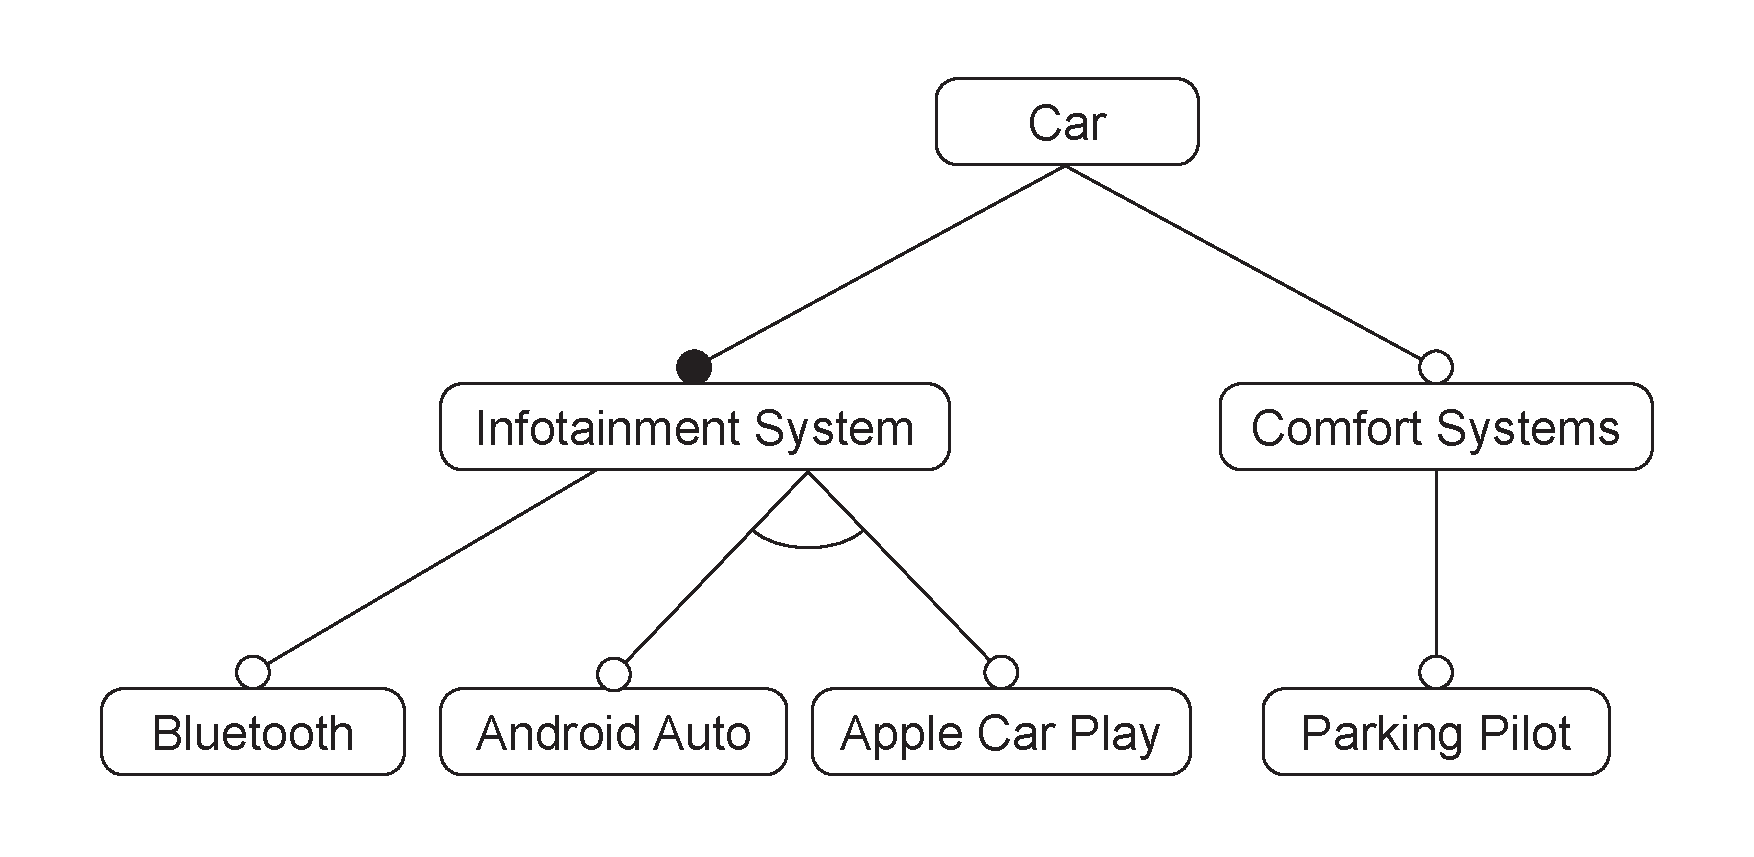
\includegraphics[width=0.8\linewidth]{illustrations/example.pdf}
	\caption{Example feature model}%
	\label{fig:example1}
\end{figure}

A visual representation of a feature model can be seen in Figure~\vref{fig:example1}. The small dot above \texttt{Infotainment System} indicates that the feature is mandatory, where as the white dot above \texttt{Comfort Systems} represents an optional feature. Each feature (except the root) is in a group. The \texttt{Infotainment System} feature is in a singleton group below \texttt{Car}. The features \texttt{Android Auto} and \texttt{Apple Car Play} are in a \texttt{XOR} group, indicated by the arch between the features. This represents that each valid variant has to choose between one of the two (but not both).

\section{Evolution planning}%
\label{sec:evolution_planning}

Feature models let engineers capture all variants of the current software product line, but sometimes it can be beneficial to model future or past versions as well. Planning for the long term evolution of the product line can be important in managing the complexity that comes with large software systems. Developing these kinds of systems typically involves many engineers, managers or other stakeholders, and managing when certain changes, additions or deprecations are implemented can be complex and confusing without suitable tools. Changing the SPL potentially influences many configurations, which might conflict with the stakeholders requirements.

SPL evolution is a major challenge in SPL engineering as many stakeholders are involved, many requirements exist, and changing the SPL potentially influences many configurations. Thus, it is paramount to thoroughly plan SPL evolution in advance, e.g., to perform analyses and to have enough time for implementing new or adapted features.

\textit{Evolution plans} lets us model a sequence of feature models, which represents the current and all planned future versions of the feature model. Each feature model represents the product line in a point in time, which could have varying validity, from a week from now to a year. Since the next feature model is derived from the previous one, we can represent the evolution plan as an initial feature model, as well as a sequence of \textit{points}, where each point is a set of operations to perform on the previous feature model to achieve the current one. The operations vary from changing, adding or deleting features or groups from the feature model.

\begin{figure}[htpb]
	\centering
	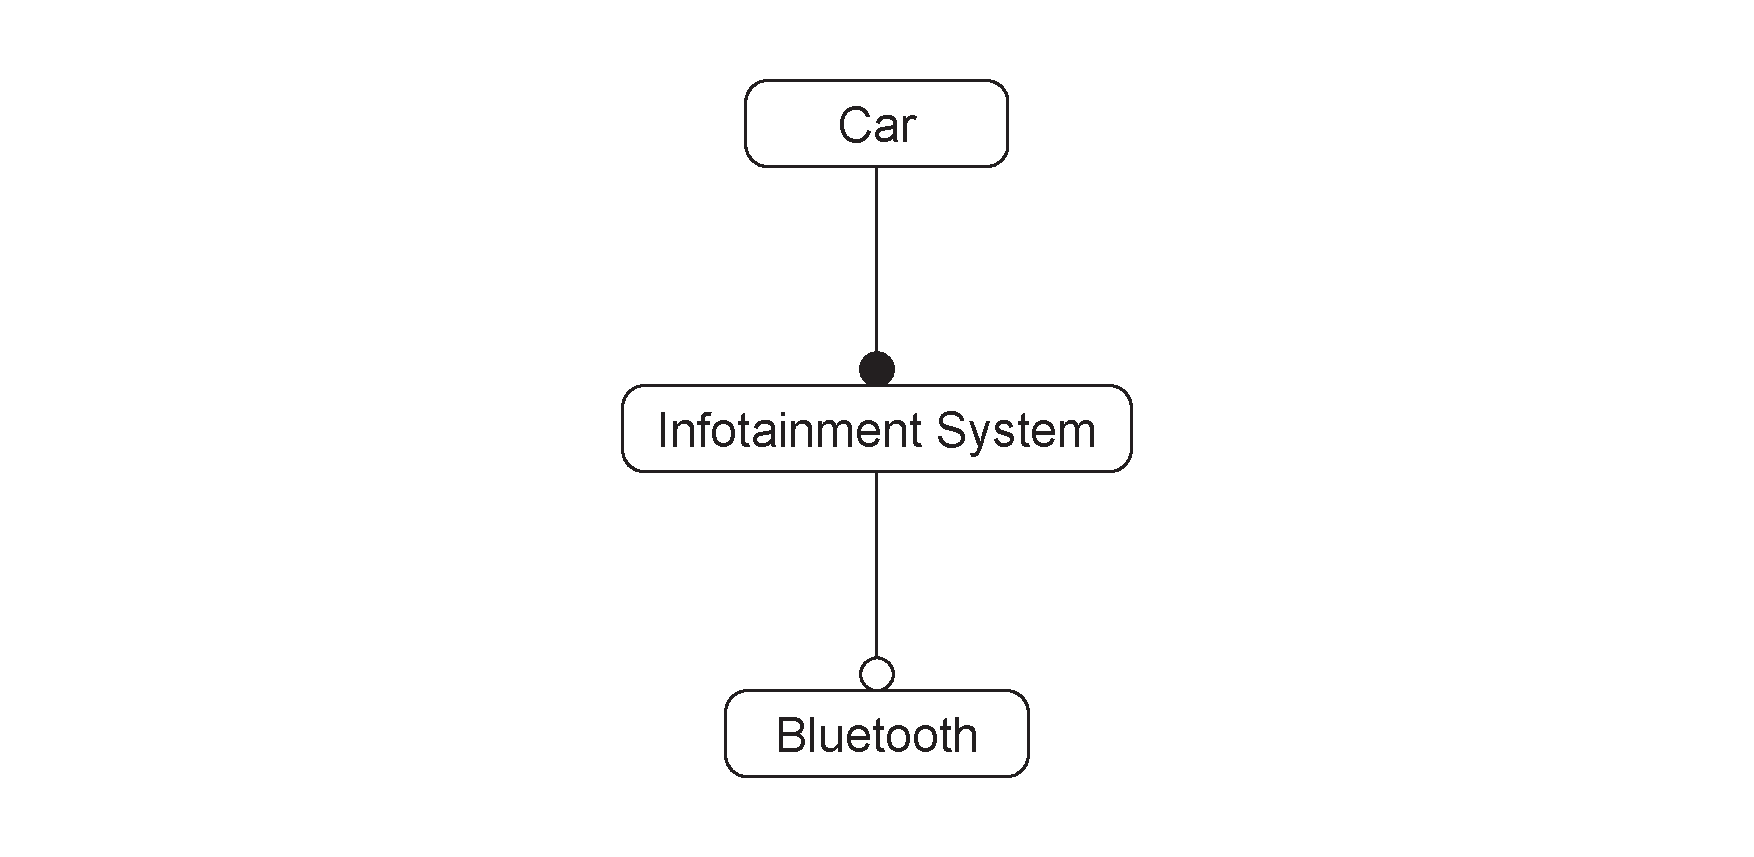
\includegraphics[width=0.8\linewidth]{illustrations/initial.pdf}
	\begin{tabular}{l}
		\textbf{At time 1:}                                           \\ \hline
		add an XOR group to Infotainment System.                      \\
		add feature Android Auto to the Infotainment System XOR group \\
		add feature Car Play to the Infotainment System XOR group     \\
		\\
		\textbf{At time 2:}                                           \\ \hline
		add feature Comfort Systems to the Car AND group              \\
		add an AND group to Comfort Systems                           \\
		add feature Parking Pilot to the Comfort Systems AND group
	\end{tabular}
	\caption{An example evolution plan}%
	\label{fig:exampleplan}
\end{figure}

An example of an evolution plan can be seen in Figure~\vref{fig:exampleplan}. The initial feature model contains three features, and two time points are added. At time 1, a group and two features are added, and at time 2, another group and two features are added. The evolution plan can derive three feature models, the initial, and the two at time 1 and 2. Performing all the operations results in a feature model that is equal to the one in Figure~\vref{fig:example1}

\section{Version Control Systems}%
\label{sec:version_control_systems}

\textit{Software configuration mechanisms} is the discipline of managing the evolution of large and complex software systems \cite{cite:software_configuration_management}. \textit{Version control mechanisms} are used to deal with the evolution of software products. These mechanisms include ways to deal with having multiple, parallel versions of the software simultaneously. Techniques like \textit{software merging} are used to keep consistency and unify different versions by automatically or semi-automatically deriving merged versions of the different parallel versions.

Mens~\cite{cite:tom_mens_software_merging_survey} categorizes and describes different aspect of version control systems and software merging techniques. Two-way and three-way merging differentiates between how many versions of the artifact you are comparing. Different representations of the merge artifact can be categorized in textual, syntactic, semantic or structural merging. State-based merge techniques uses delta algorithms to compute differences between revisions while change-based techniques keeps track of the exact operations that were performed between the revisions.

\subsection{Two-way vs three-way merging}%
\label{sub:two_way_vs_three_way_merging}

When merging different versions of a piece of software, we differentiate between \textit{two-way} and \textit{three-way} merging. Two-way merging merges the two versions without taking a common ancestor into account. Three-way merging on the other hand, uses a common ancestor as a reference point, to know how the different versions were changed. The latter technique is more powerful and produces more accurate merges, because the merge will know extra information from the common ancestor.

To illustrate the difference, consider the following program: \texttt{print(a); print(b); print(a + b)}, and two different versions derived from the base program, (1) \texttt{print(a); print(b); print(a+b); print("new line")}, (2) \texttt{print(b); print(a + b)}. Since a three-way merger uses the base program as a reference point, it will notice that derived version 1 added one statement, while version two deleted one. The three-way merger will then merge successfully without conflict with the following result: \texttt{print(b); print(a + b); print("new line")}. However, a two-way merger does not use the base program the different versions were derived from, and can not deduce whether \texttt{print(a)} were added in version 1 or deleted in version 2, thus raising a conflict. The same ambiguity occurs with the added statement \texttt{print("new line")}.

\subsection{Textual merging}%
\label{sub:textual_merging}

Textual merging views the software artifacts as unstructured text files. There exist several granularities of what is considered one unit, but \textit{line-based merging} is probably the most common textual merge. Line-based merging techniques computes the difference between files by comparing equality over the lines. This has several implications, like adding a single space after a line is considered a deletion of the old line and addition of the new. This coarse granularity often leads to unnecessary and confusing conflicts. Changing the indentation or other formatting differences often lead to unnecessary conflicts.

To exemplify this, consider the two versions of a Python program, Listing~\vref{lst:code_diff_1} and Listing~\vref{lst:code_diff_2}. The second version simply wrapped the content of the function in an if-statement that checks for input sanity. Using a standard textual, line-based differencing tool like the Unix' \textit{diff}-tool \cite{cite:fast_algo_for_lcs}, we are able to calculate the difference between the two files by calculating the longest common subsequence. As seen in the result (Listing~\vref{lst:result_code_diff}), difference between the two are confusing and inaccurate. Conceptually, the difference is that the second version wrapped the block in a if-statement. Due to the coarse grained line-based differencing and the disregard of structure and semantics, the algorithm reports that the whole block is deleted, and the same block wrapped in an if is inserted.

\begin{listing}
	\begin{minted}[]{python}
def some_function(n):
  sum = 0
  for i in range(0, n):
    sum += i
  print(sum)
some_function(5)

  \end{minted}
	\caption{Code diff 1}
	\label{lst:code_diff_1}
\end{listing}

\begin{listing}
	\begin{minted}[]{python}
def some_function(n):
  if isinstance(n, int):
    sum = 0
    for i in range(0, n):
      sum += i
    print(sum)
some_function(5)
  \end{minted}
	\caption{Code diff 2}
	\label{lst:code_diff_2}
\end{listing}

\begin{listing}
	\begin{minted}{text}
<   sum = 0
<   for i in range(0, n):
<     sum += i
<   print(sum)
---
>   if isinstance(n, int):
>     sum = 0
>     for i in range(0, n):
>       sum += i
>     print(sum)
  \end{minted}
	\caption{Resulting code diff}
	\label{lst:result_code_diff}
\end{listing}

As discussed, text-based merge techniques often provide inferior results, however, they have several advantages in terms of efficiency and generality. The algorithm is general enough to work well for different programming languages, documentation, markup files, configuration files, etc. Some measurements performed on three-way, textual, line-based merge techniques in industrial case studies showed that about 90 percent of the changed files could be merged automatically \cite{cite:large_scale_case_study}. Other tools can complement the merge algorithm in avoiding or resolving conflicts. Formatters can make sure things like indentation and whitespace are uniformly handled, to avoid unnecessary conflicts. Compilers can help in resolving conflicts arising from things like renaming, where one version renames a variables, while another version introduces new lines referencing the old variable.

\subsection{Syntactic Merging}%
\label{sub:syntactic_merging}

\textit{Syntactic merging}~\cite{cite:syntactic_software_merging} differs from textual merging in that it considers the syntax of the artifact it is merging. This makes it more powerful, because depending on the syntactic structure of the artifact, the merger can ignore certain aspects, like whitespace or code comments. Syntactic merge techniques can represent the software artifacts in a better data structure than just flat text files, like a tree or a graph. In example, representing the Python program from Listing~\vref{lst:code_diff_1} and Listing~\vref{lst:code_diff_2} as a parse tree or abstract syntax tree, we can avoid merge conflicts.

The granularity of the merger is still relevant, because we sometimes want to report a conflict even though the versions can be automatically merged. Consider the following example. $n < x$ is changed to $n \leq x$ in one version, and to $n < x + 1$ in another. Too fine grained granularity may cause this to be merged conflict free as $n \leq x + 1$. The merge can be done automatically and conflict free, but here we want to report a warning or conflict, because the merge might lead to logical errors.

\subsection{Semantic Merging}%
\label{sub:semantic_merging}

While syntactic merging is more powerful than its textual counterpart, there are still conflicts that go unnoticed. The syntactical mergers can detect conflicts explicitly encoded in the tree structure of the software artifact, however, there often exist implicit, cross-tree constraints in the software. An example of such a constraint is references to a variable. The variable references in the code are often semantically tied to the definition of the variable, where the name and scope implicitly notes the cross tree reference to the definition.

Consider the following simple program: \texttt{var i; i = 10;}. If one version changes the name of the variable: \texttt{var num; num = 10;}, and another version adds a statement referencing the variable: \texttt{var i; i = 10; print(i)}. Syntactic or textual mergers would not notice the conflict arising due to the implicit cross-tree constraints regarding the variable references, and merge the versions conflict-free with the following, syntactically valid result: \texttt{var num; num = 10; print(i)}.

Semantic mergers takes these kinds of conflicts into consideration while merging. Using \textit{Graph-based}  or \textit{context-sensitive} merge techniques, we can model such cross tree constraints, by linking definitions and invocations with edges in the graph. However, in some cases, such \textit{static semantic} merge techniques are not sufficient. Some changes cannot generally be detected statically, and may need to rely on the runtime semantics.

\section{Haskell and Algebraic Data Types}%
\label{sec:haskell_and_algebraic_data_types}

\chapter{Formal Semantics of Feature Model Evolution Plans}%
\label{cha:formal_semantics_of_feature_model_evolution_plans}

\chapter{Three Way Merge Algorithm}%
\label{cha:three_way_merge_algorithm}

\section{Algorithm Overview}%
\label{sec:algorithm_overview}

\subsection{Three-Way Merging of Evolution Plans}%
\label{sub:three_way_merging_of_evolution_plans}

The three-way merge algorithm for feature model evolution plans will take two different versions of an evolution plan, \textit{version 1} and \textit{version 2}, and attempt to merge the evolution plans into a single plan. In order to do so, a third evolution plan has to be provided, which is the common evolution plan they were derived from. The common evolution plan, called \textit{base}, will implicitly provide information about what things were added, removed and changed in each of the derived evolution plans.

\subsection{Soundness Assumption}%
\label{sub:soundness_assumption}

The three-way merge algorithm will assume that the three evolution plans provided are sound. By assuming the soundness of the plans, the algorithm can leverage this to create a better merge result. But more importantly, the assumption is based around the fact that there is no point in merging an evolution plan you know violates soundness in some way.

\subsection{Algorithm Phases}%
\label{sub:algorithm_phases}

In order to merge the different versions of the evolution plan, the algorithm is separated into several distinct phases. The different steps and phases of the algorithm can be seen in Figure~\ref{fig:merge_outline}.

\begin{figure}[htbp]
  \centering
  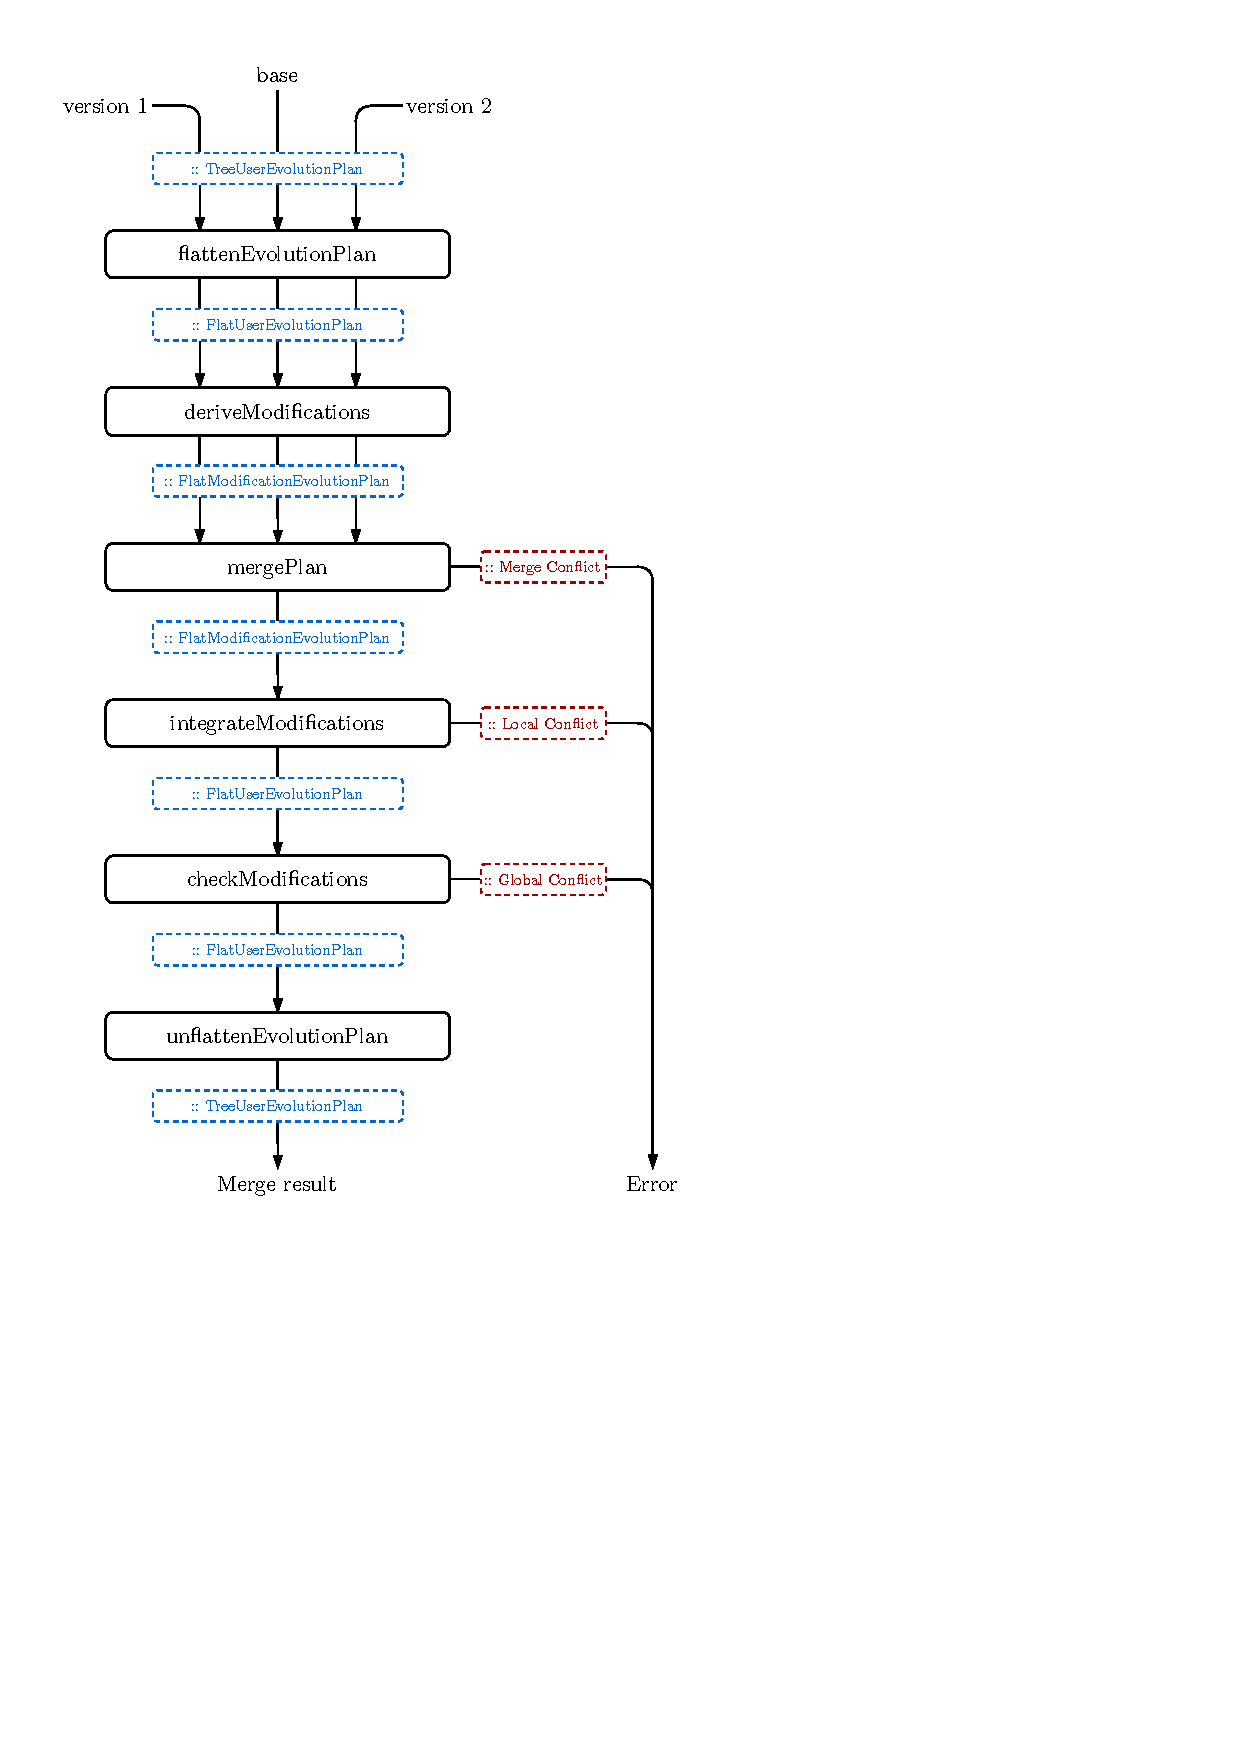
\includegraphics[width=0.8\linewidth]{merge_outline}
  \caption{Outline of the three-way merge algorithm}%
  \label{fig:merge_outline}
\end{figure}

The first phase is transforming the three different evolution plans into representations that is more suitable for merging. This includes converting both the way feature models are represented as well as the way the entire evolution plan is represented. This phase includes the \texttt{flattenEvolutionPlan} and \texttt{deriveModifications}, which is described in further detail in \vref{sec:converting_to_a_suitable_representation}

After changing the way evolution plans are represented, the second phase of the algorithm will calculate the differences between the \textit{base} evolution plan and both derived evolution plans, \textit{version 1}, and \textit{version 2}. This will let us know what were added, changed and removed in each of the derived evolution plans. This phase is part of the \texttt{mergePlan} function, which is described in further detail in \vref{sec:detecting_the_changes_between_versions}

The information from the previous phase will be used to create a single merged evolution plan. This evolution plan is simply just the \textit{base} evolution plan integrated with all the changes from \textit{version 1} and \textit{version 2}. This phase is part of the \texttt{mergePlan} function, which is described in further detail in \vref{sec:merging_intended_changes}

Now that a single merged evolution plan is provided, the last step is to ensure that the plan is following the structural and semantic requirements of an evolution plan. Merging all changes from both versions might yield various inconsistencies. This includes structural conflicts such as orphan features, entire subtrees forming cycles, removing non-empty features, etc. The last phase includes converting back to the original representation, as well as ensuring soundness while doing so. This phase is part of the \texttt{integrateModifications}, \texttt{checkModifications} and \texttt{unflattenEvolutionPlan} functions, which is explained further in \vref{sec:ensuring_structural_and_semantic_soundness_of_merge_result}

\subsection{Conflicts}%
\label{sub:conflicts}

During the different phases of the merge algorithm, different kind of conflicts or errors could occur. Depending on what part of the algorithm a conflict occurred, the conflicts might be either a \textit{merge}, \textit{local} or \textit{global} conflict. For example, if both versions perform different operations on the same feature at the same time point, the 

\section{Converting To a Suitable Representation}%
\label{sec:converting_to_a_suitable_representation}

\subsection{Representing Feature Models}%
\label{sub:representing_feature_models}

\subsection{Representing Evolution Plans}%
\label{sub:representing_evolution_plans}

\section{Detecting the Changes Between Versions}%
\label{sec:detecting_the_changes_between_versions}

\section{Merging Intended Changes}%
\label{sec:merging_intended_changes}

\section{Ensuring structural and semantic soundness of the merge result}%
\label{sec:ensuring_structural_and_semantic_soundness_of_merge_result}

\chapter{Conclusion and Future Work}%
\label{cha:conclusion_and_future_work}

\backmatter{}

\printbibliography

\end{document}
